%!TEX root = ../template.tex
%%%%%%%%%%%%%%%%%%%%%%%%%%%%%%%%%%%%%%%%%%%%%%%%%%%%%%%%%%%%%%%%%%%
%% chapter1.tex
%% NOVA thesis document file
%%
%% Chapter with introduction
%%%%%%%%%%%%%%%%%%%%%%%%%%%%%%%%%%%%%%%%%%%%%%%%%%%%%%%%%%%%%%%%%%%

\typeout{NT FILE chapter1.tex}%

\chapter{Introduction}
\label{cha:introduction}

In this chapter, we will present the motivation and problem statement that led
to the development of this dissertation, highlighting the global health
challenge posed by breast cancer and the potential of microRNAs as biomarkers
for its classification. We will also outline the challenges and research
hypothesis that guide this work, as well as the expected contributions and
organization of the document.

\section{Motivation \& Problem Statement}
\label{sec:motivation+problem-statement}
\subsection{Breast Cancer - A Global Health Challenge}

\gls{bc} is currently one of the biggest public health challenges worldwide. In
2022, an article from \textcite{bcaData2024_bray} showed that more than $2.3$
million new cases of \gls{bc} were diagnosed, resulting in
around $665,\!000$ global deaths . Other studies
estimate that \gls{bc} will continue to not only bethe most commonly diagnosed
cancer but also to increase in incidence, with projections indicating that by
2040, the number of deaths will almost double and the number of new cases will
be around $3.2$ million \cite{bca_data_Arnold2022Current}. Figure
\ref{fig:estimates_2020_2040} and \ref{fig:graphic_incidencies_world}
underline the high incidence and mortality associated with the disease,
highlighting the geographical variations in disease burden and the ongoing need
to develop more effective strategies for its diagnosis and treatment.

\begin{figure}[h!]
  \centering
  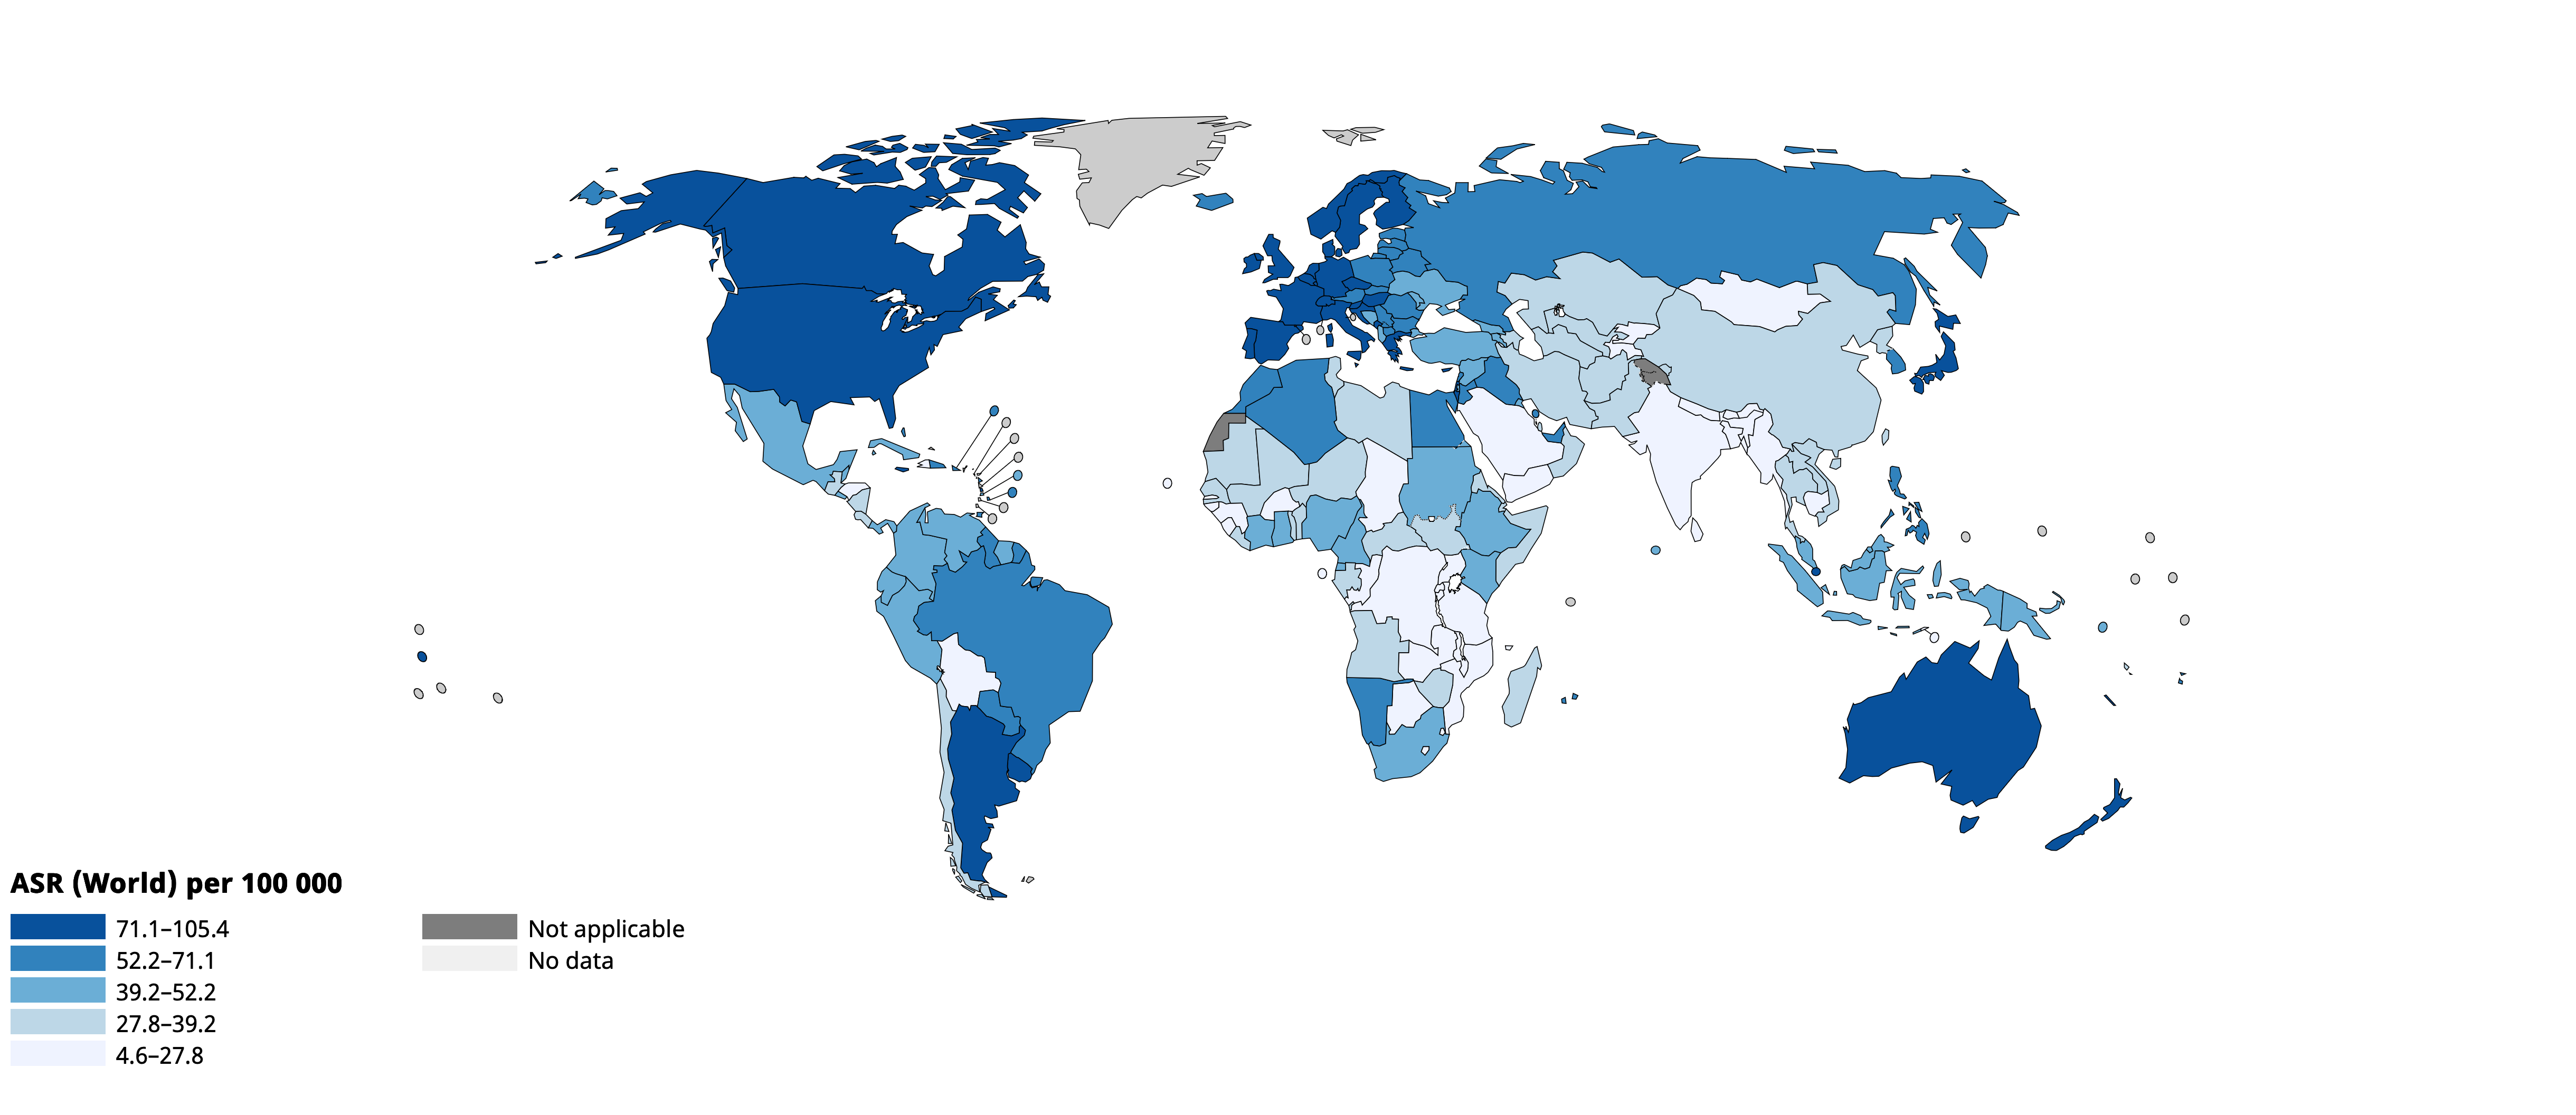
\includegraphics[width=1.0\textwidth]{/Users/JoseRomano/Documents/Tese/bca-thesis/Chapters/Figures/graphic_incidencies_world.png}
  \caption{Age-standardized incidence rate (ASR, per 100,000 inhabitants) of breast cancer in both sexes in 2022.
    The data represent global estimates based on \textcite{GLOBOCAN2022}.}
  \label{fig:graphic_incidencies_world}
\end{figure}

\begin{figure}[h!]
  \centering
  \begin{subfigure}[b]{0.45\textwidth}
    \centering
    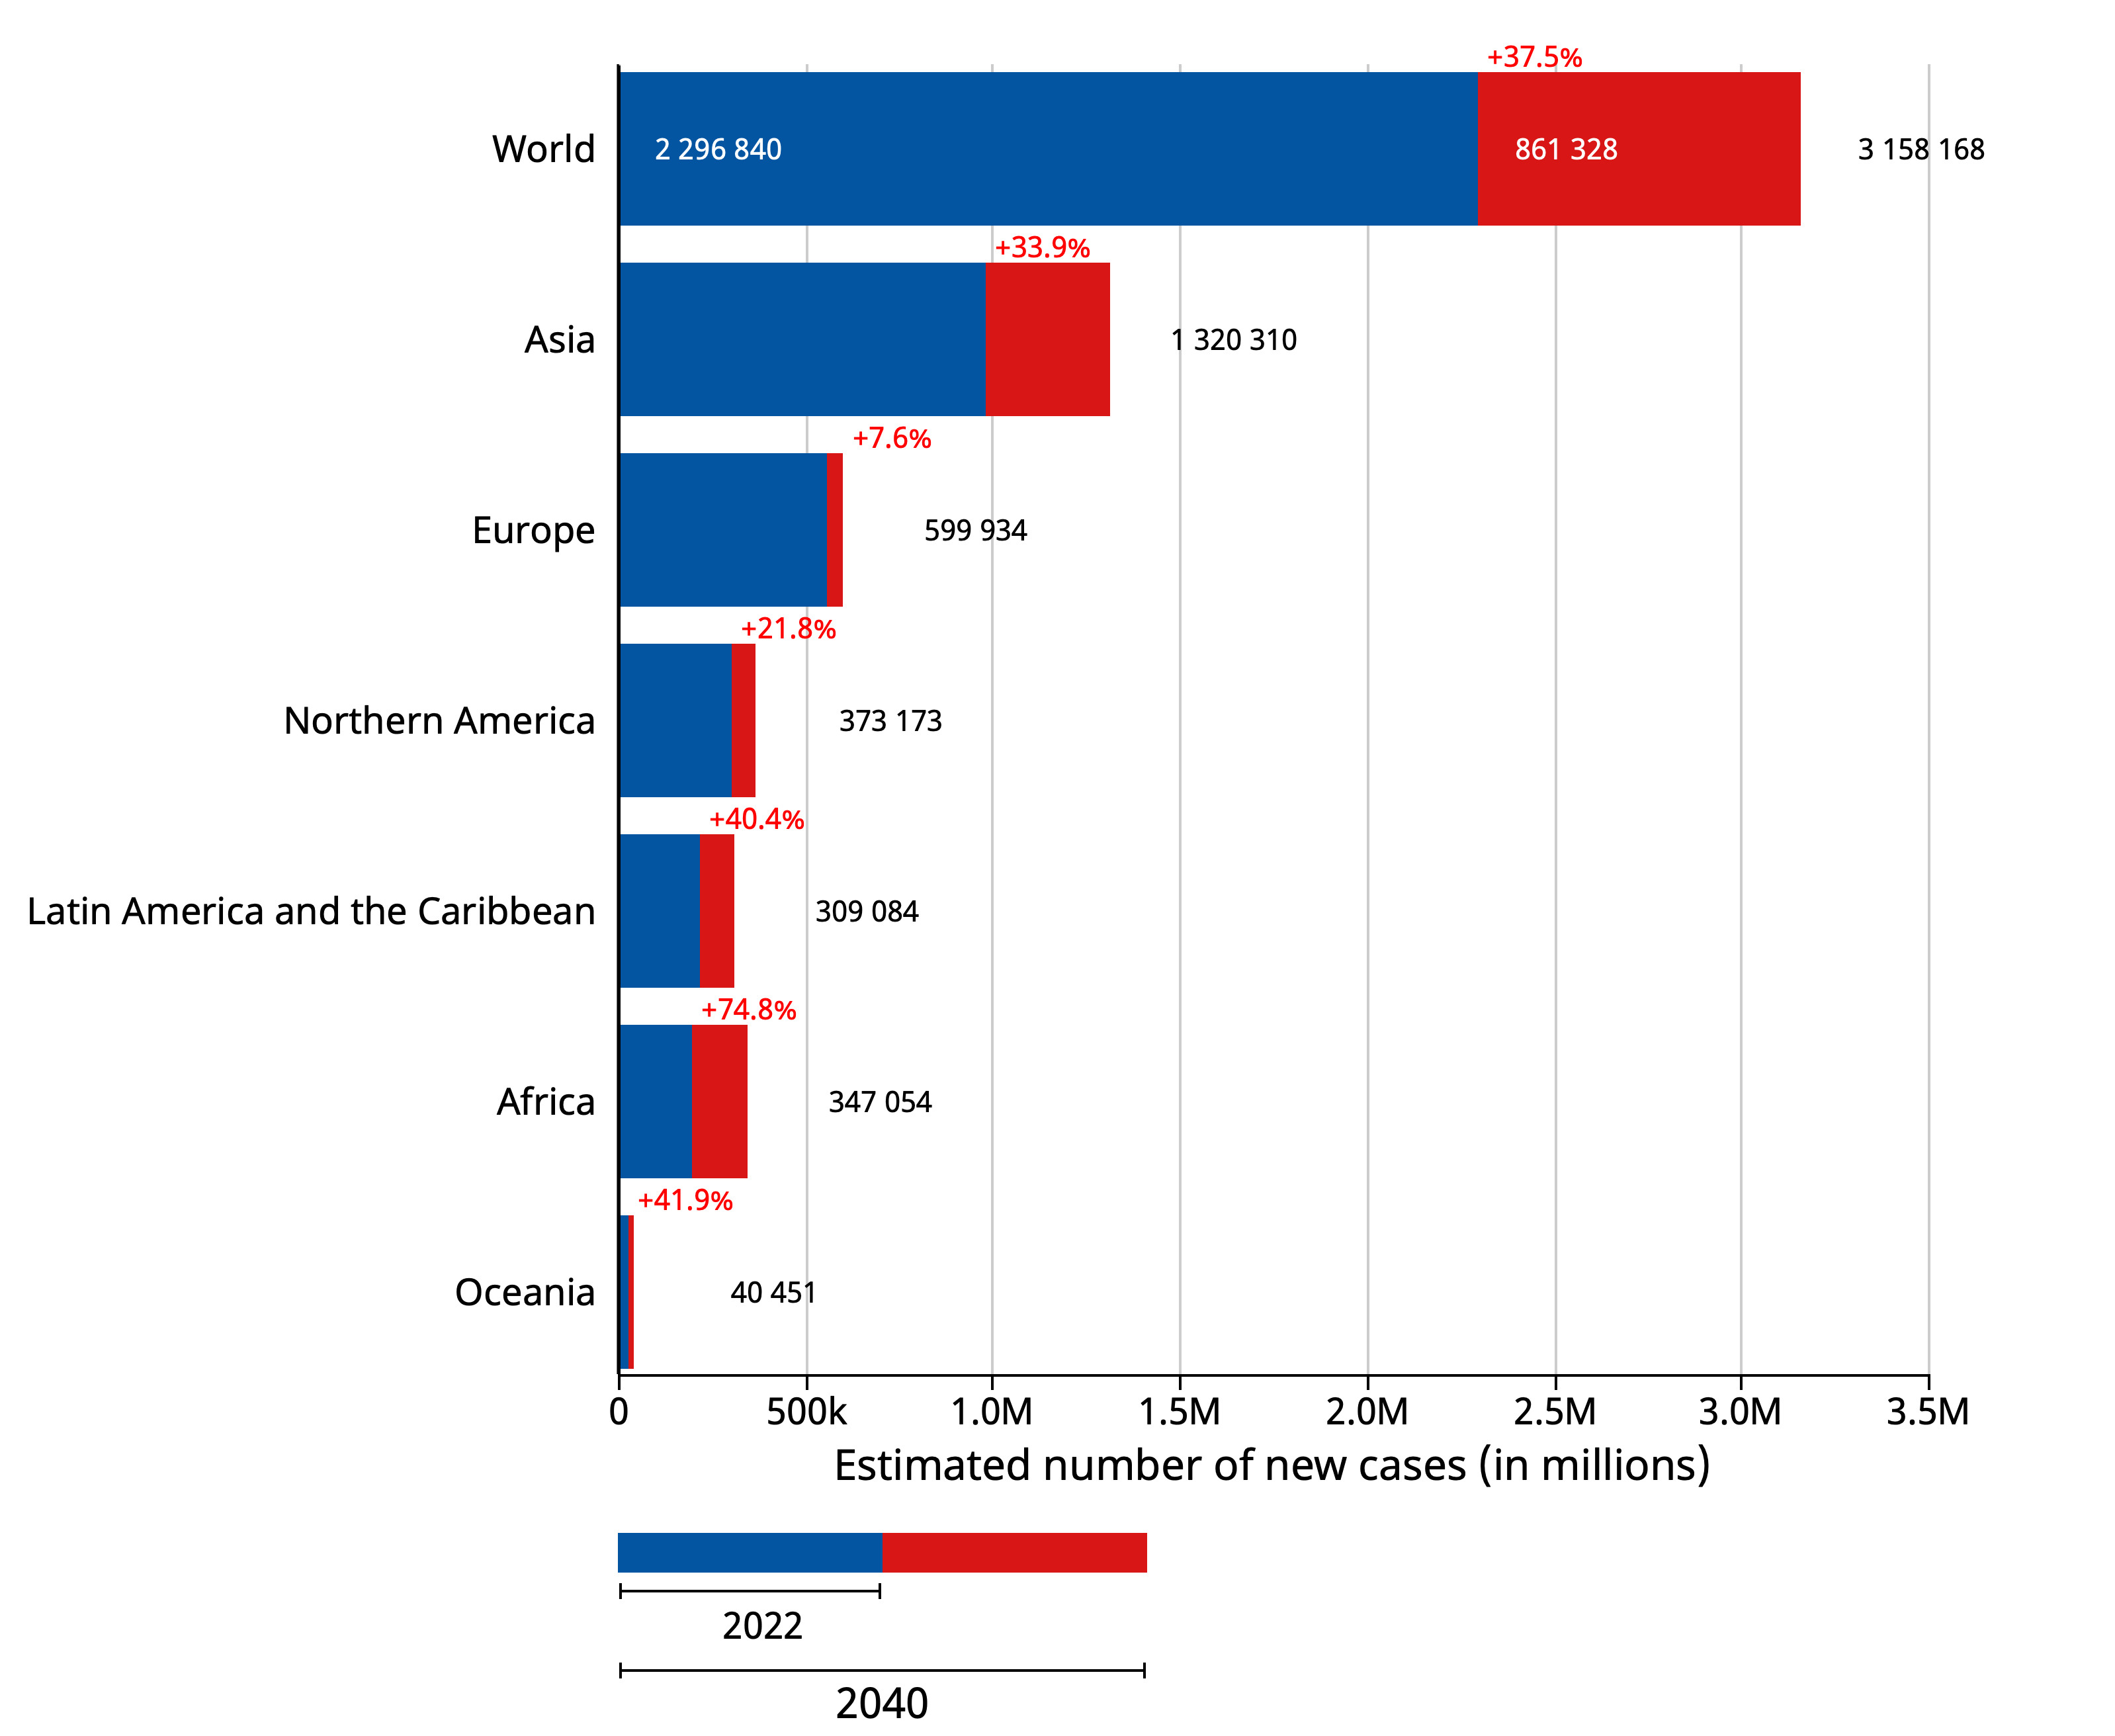
\includegraphics[width=\textwidth]{/Users/JoseRomano/Documents/Tese/bca-thesis/Chapters/Figures/new_cases_2020_2040.png}
    \caption{Estimate number of new cases of Breast Cancer}
    \label{fig:new_cases_2020_2040}
  \end{subfigure}
  \vspace{0.5cm}
  \begin{subfigure}[b]{0.45\textwidth}
    \centering
    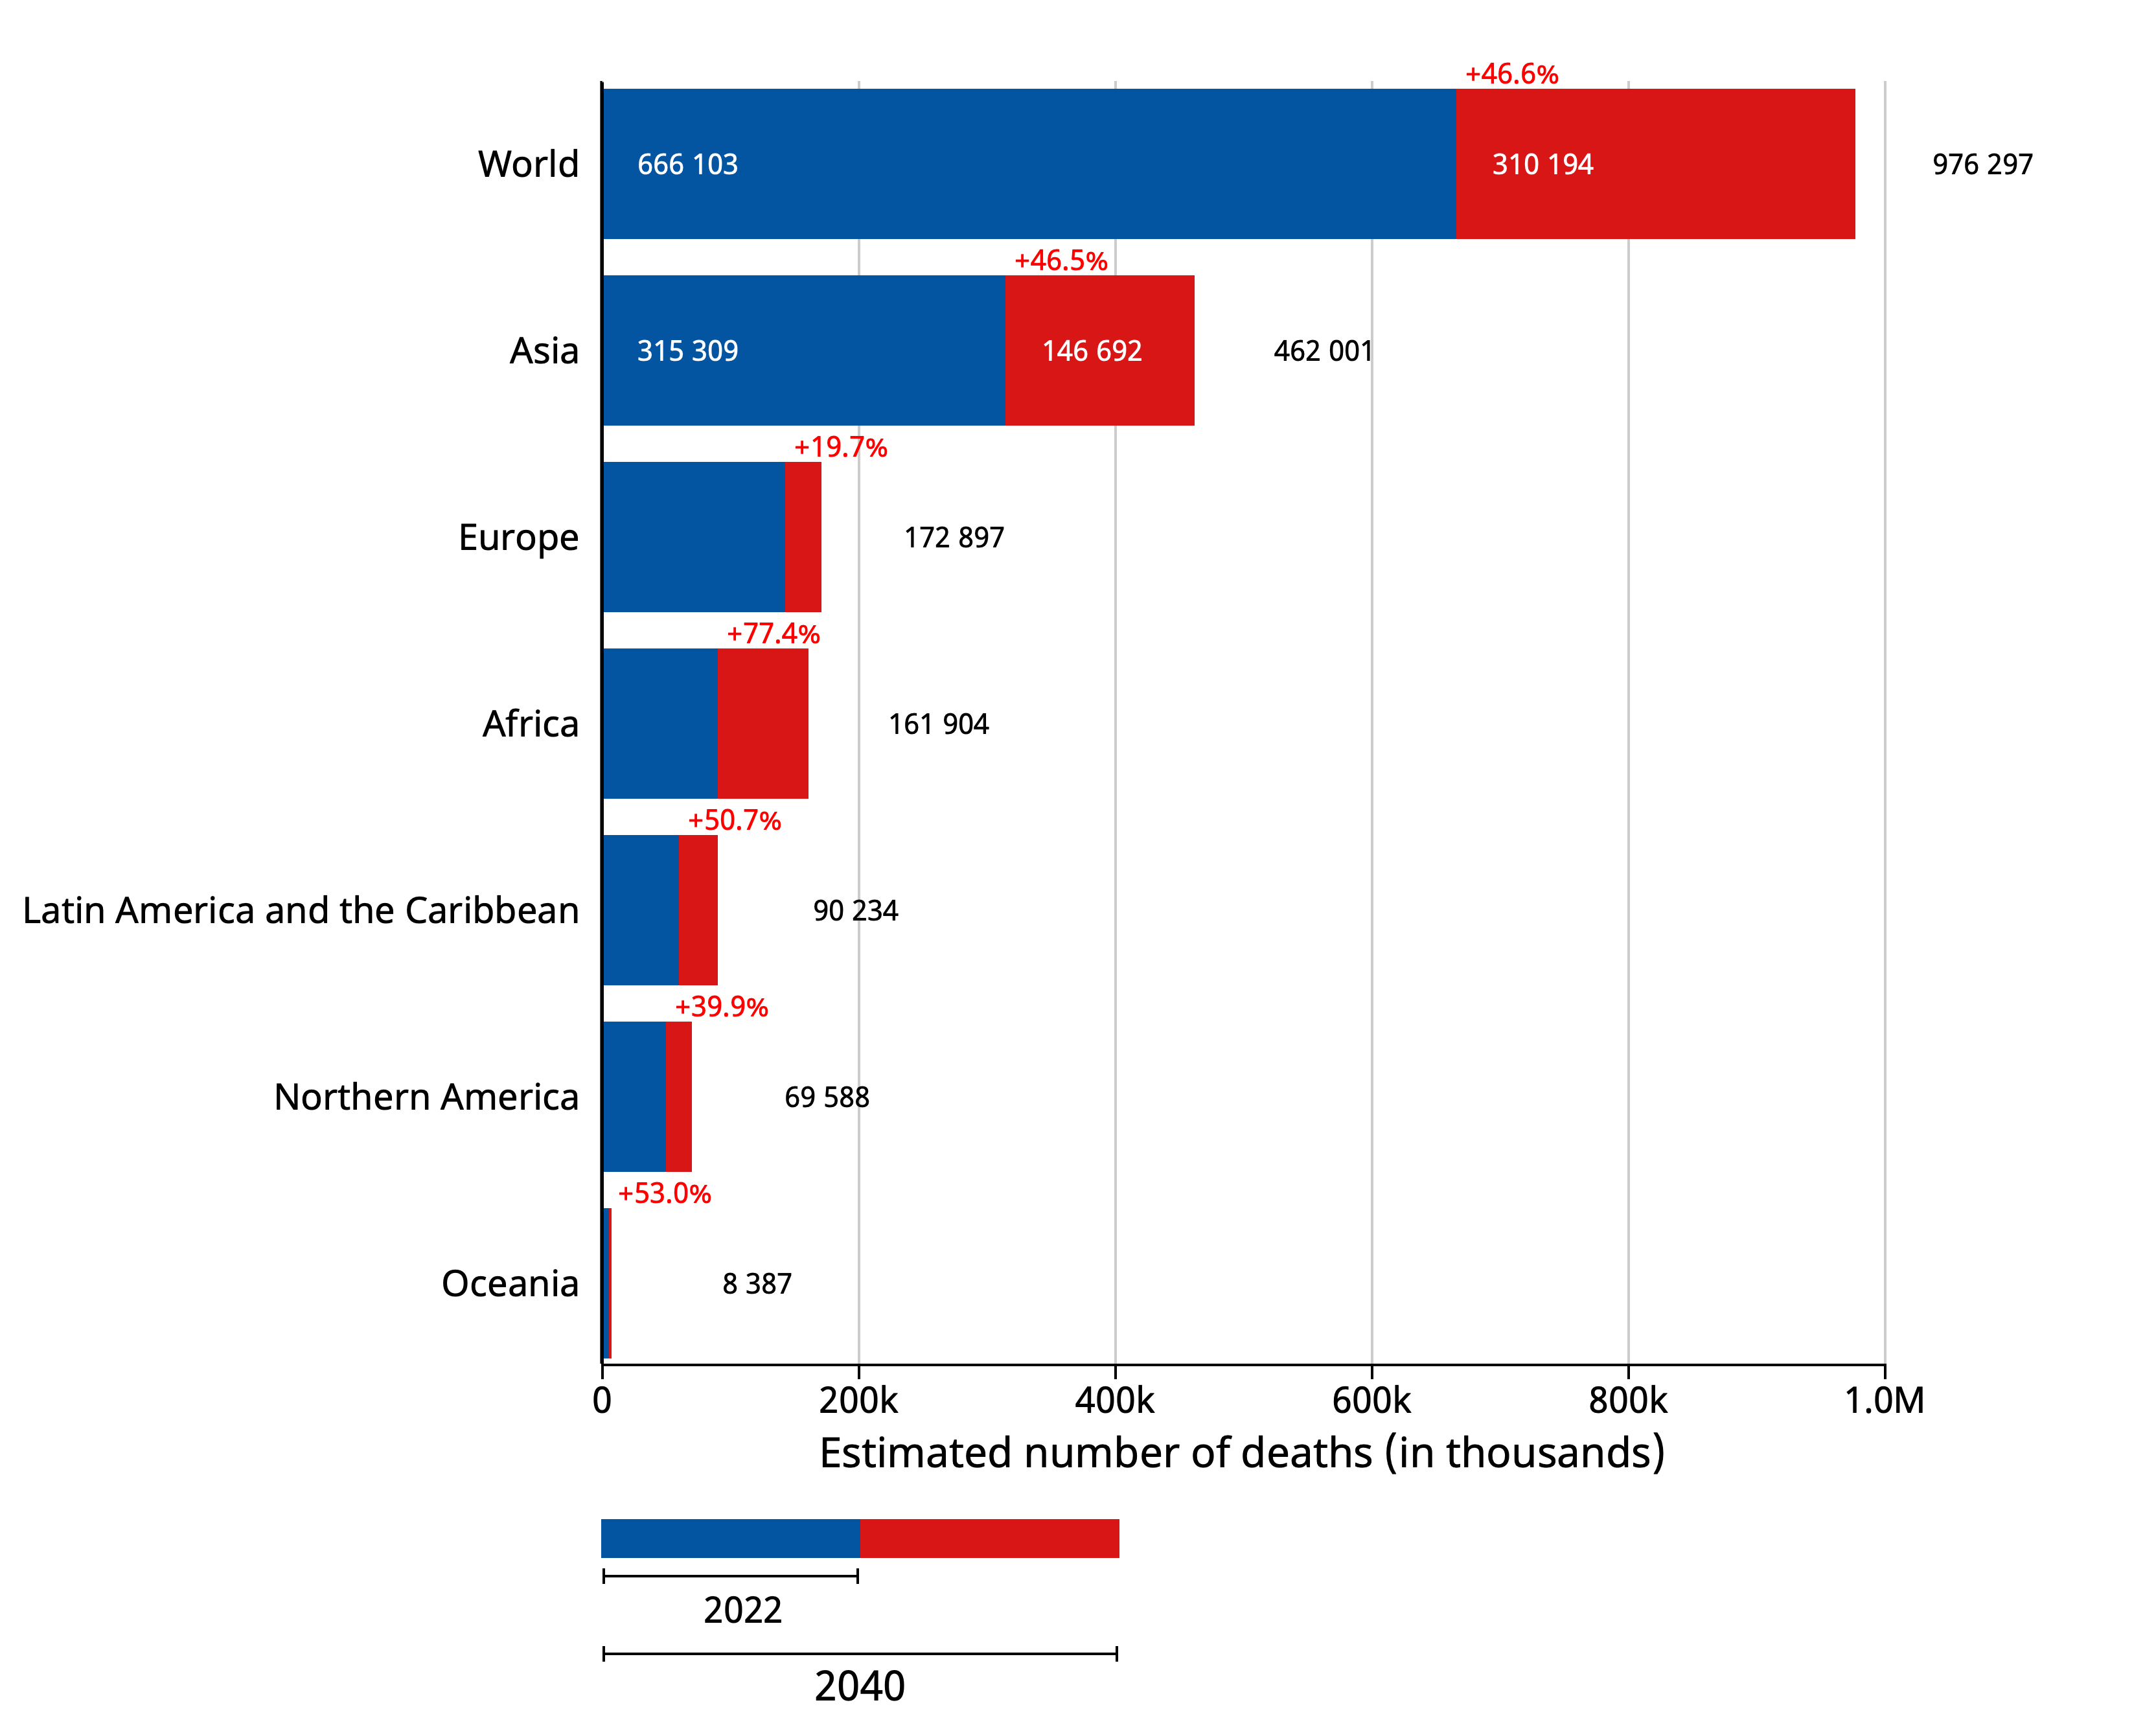
\includegraphics[width=\textwidth]{/Users/JoseRomano/Documents/Tese/bca-thesis/Chapters/Figures/deaths_2020_2040.png}
    \caption{Estimate number of deaths caused by Breast Cancer}
    \label{fig:deaths_2020_2040}
  \end{subfigure}
  \caption{Visual comparison of the estimated number of new cases and deaths caused by Breast Cancer
    in 2020 (in blue) and 2040 (in red). \cite{GLOBOCAN2022}}
  \label{fig:estimates_2020_2040}
\end{figure}

BC is characterized by marked biological heterogeneity, manifested in multiple
molecular subtypes that exhibit distinct clinical behaviors . Each subtype
exhibits substantial differences in terms of tumor aggressiveness, metastatic
potential, and behavior to specific therapies as demonstrated by
\textcite{bc_subtypes_Prat2015Clinical} and \textcite{bc_molecular_Perou2000}.
However, in the work of \textcite{need_for_subtype_treatments_Testa2020Breast},
we get a comprehensive explanation of why accurate classification of these
subtypes is essential to enable personalized therapeutic approaches, with a
direct impact on treatment efficacy and disease prognosis.

\subsection{Can we improve the classification of Breast Cancer subtypes?}
Among the emerging candidates for robust biomarkers for the classification of
\gls{bc} subtypes are \gls{mirna}, small non-coding RNA molecules that play a
crucial regulatory role in gene expression. They are estimated to modulate the
expression of about one-third of the genes in the human genome
\cite{mirna_importance_Hammond2015An} and are implicated in the regulation of
multiple physiological and pathological processes, including various human
diseases \cite{mirna_as_biomarkers_Ho2022}.

Given their regulatory nature, several studies have demonstrated a significant
association between \gls{mirna} expression profiles and relevant clinical
characteristics in the context of \gls{bc}, including processes such as tumor
progression and metastasis development, as seen in
\textcite{_Mendes2022Nanodelivery} \textcite{mirna_as_biomarkers_Ho2022} and
\textcite{mirnas_in_bc_Muñoz2023}. In addition to these aspects, a seminal
study by \textcite{mirna_as_bio_for_sub_Blenkiron2007MicroRNA} demonstrated
that \gls{mirna} expression profiles can effectively distinguish between
different molecular subtypes of \gls{bc}, highlighting their potential as a
precise subtyping tool. This ability to discriminate between subtypes
reinforces the value of \gls{mirna} as promising clinical biomarkers.

\subsection{How to identify the most relevant miRNAs?}

The identification of the most relevant \gls{mirna} for \gls{bc} profilling
represents a major analytical challenge due to the complexity of these high
dimensional regulatory molecules, non-linearity interactions between and
clinical phenotypes that require advanced computational approaches to be
effectively modelled. Recent advances in \gls{ai}, some of which are explored
in the work of \textcite{ml_for_microRNA_Luo2023MachineLearning},particularly
in \gls{ml} and \gls{dl}, have demonstrated remarkable potential in extracting
meaningful patterns from high-dimensional and heterogeneous (data from distinct
nature) biomedical data. These approaches enable not only the accurate
classification of \gls{bc} subtypes but also the identification of
discriminative \gls{mirna} signatures, supporting their integration as
actionable biomarkers in clinical workflows.

In this context, \gls{ml} and \gls{dl} models are particularly well suited for
the task of robustly characterizing and explaining the profiles of
\gls{mirna}-based biomarkers — should such biomarkers exist — with the
potential to effectively discriminate between different \gls{bc} subtypes, as
already seen in a study done by \textcite{ml_gastric_Azari2023} where \gls{ml}
algorithms identified potential diagnostic and prognostic \gls{mirna} in
gastric cancer, showing high accuracy in the identification of reliable
biomarkers for this disease.

This reality reinforces the urgency of developing advanced computational tools
that can enable more precise molecular characterization and guide personalized
therapeutic decisions, ultimately improving clinical outcomes for patients with
aggressive and hard-to-treat \gls{bc} subtypes.

\section{Challenges and research hypothesis}
\label{sec:challenges+research-hypothesis}
Based on the assumption that it is possible to use microRNA expression values
and clinical data to map \gls{bc} subtypes, as shown by
\textcites{mirna_as_biomarkers_Ho2022}{mirnas_in_bc_Muñoz2023}, this dissertation
proposes to explore several complementary directions for this pathology where
the application of \gls{ai} techniques is still growing.

First, we intend to assess whether discriminative linear models perform better
than latent representation models (in a context where there are two different
data sources and many dimensions) - such as DIABLO \cite{DIABLO_Singh2019}, a
widely used model. At the same time, we will investigate the impact of patient
clinical information (such as age, presence or absence of metastases, hormone
levels, among others) on the classification performance of the models, where we
will be able to gain valuable insights into possible relationships between
these features and \gls{bc} subtypes.

If substantial results are obtained by any of the models, we will be able to
conduct a more extensive study on our main point: whether or not there are
\gls{mirna} that are potential biomarkers for \gls{bc} subtypes. In a more
advanced approach, I will be able to explore the applicability of
\textit{Conformal Prediction} \cite{conformal_prediction_Angelopoulos2023},
which provides statistically based confidence intervals for each prediction
(which is widely used in areas where risk must be justified and well-founded,
such as finance and healthcare) \cite{conformal_prediction_Angelopoulos2023}.
The latter is an approach that is still gaining ground in healthcare and,
considering our problem, it makes sense to be able to give a prediction based
on a confidence interval, giving our model greater transparency and
reliability, something particularly relevant in clinical contexts where error
must be minimized and uncertainty well characterized.

Even though the base seems promising, there are several challenges to overcome
in order to achieve the desired results such as: \\ \textbf{1. Biological
  heterogeneity:} \\ \label{sec:biological-heterogeneity} Biological
heterogeneity is characterized by the diversity of living organisms, including
species, genotypes, and populations, which exhibit a variety of biological
characteristics, such as morphology, physiology, genetics, and biogeography.
The human body is a highly complex system in which the behavior of each
component depends on its interaction with countless other parts. Exposure to
the same treatment by two bodies can result in completely different reactions.
\\ \textbf{2. Functional complexity of microRNAs:} \label{sec:mirna_complexity}
\\ The role of \gls{mirna} in biological regulation and cancer progression is
extremely complex and still relatively new from a scientific point of view. The
action of a single microRNA is not isolated, but rather part of a network of
interactions with dozens (or hundreds) of other \gls{mirna} and contextual
factors. This highly interdependent behavior raises questions about the
effectiveness of overly simplistic or linear models. The application of
nonlinear models allows for the discovery of complex relationships and
cross-interactions between different \gls{mirna} or between them and clinical
variables. These relationships and interactions would be invisible to more
traditional approaches. \\ \textbf{3. No control set:} \\ Another relevant
challenge is the absence of a control set that includes data from healthy
individuals. Since this type of analysis (\gls{mirna} expression profiling) is
not routinely performed in individuals without cancer, it is difficult to
define what would be a “normal level” of expression. The implementation of a
control group would not only broaden the scope of the model's task (e.g.,
distinguishing between the presence and absence of cancer before predicting the
subtype), but also optimize the robustness of biomarker identification. An
illustrative example of this phenomenon is presented in the study
\textcite{ml_gastric_Azari2023} where the implementation of a control set was
fundamental to the identification of discriminative markers.

The data for this study were previously selected by Dr. Bárbara Mendes and her
team based on purely biological selection criteria. These criteria included the
scientific interest of the group and molecular characteristics that were
considered relevant in the context of the research. Consequently, the dataset I
was given consists of 256 biopsies and 888 \gls{mirna} features, as well as 38
clinical data features. This presents a scenario of high dimensionality with a
limited number of examples on which to train.

The morphology of this dataset limits the choice of approaches to be used and
requires extra caution in how we work with certain models, such as nonlinear
ones, given their high adaptability in high dimensions, which, in a context of
limited data, can easily lead to overfitting. This requires careful selection
of algorithms and attention to the pipeline that is set up to ensure that the
results obtained are robust and relevant.

Furthermore, this problem cannot be addressed with data augmentation techniques
used in the field of \gls{ml}, such as \textit{SMOTE} (Synthetic Minority
Over-sampling Technique - \textcite{SMOTE_Blagus2013SMOTE}). As discussed
earlier in the topic \ref{sec:biological-heterogeneity}, the nature of this
data makes reliable synthetic generation unfeasible, which can lead to
artificially inconsistent samples ("Extra-terrestial beings", in other words).

A control set would be an important step toward increasing the generalizability
of our model. This data set would not only allow us to expand the problem to
include the distinction between healthy and sick individuals, but also improve
the identification of discriminative biomarkers. The latter has already been
successfully tested in other types of cancer, and a key step in the pipeline
used is precisely the comparison with a control set \cite{ml_gastric_Azari2023}
to isolate clinically relevant markers.

\section{Expected Contributions}
\label{sec:expected-contributions}
The main contribution of this dissertation is the development of a computational
framework for the classification of \gls{bc} subtypes based on \gls{mirna}
expression and patient clinical data. This framework will integrate
and compare different \gls{ml} and \gls{dl} approaches (still underexplored for this decease)
applied to a problem of high biological and statistical complexity.

In addition to the classification process, this framework will include a
statistical analysis component aimed at validating the predictions made in
order to give robustness to the decision made by the model. This robustness is
particularly relevant in a clinical setting, where transparency and reliability
of predictions are essential for possible future translation into medical
practice and the findings of this work will be tested using \textit{in-vivo}
methods by the team of Dr. Bárbara Mendes in NOVA Medical School.

Throughout the work, a critical and comparative analysis of the approaches
explored will be promoted, focusing on their applicability to complex and
heterogeneous biomedical data. It is thus hoped to contribute to the
development of more robust, explainable computational solutions adapted to the
reality of biological systems, reinforcing the potential of \gls{mirna} as
relevant molecular markers in the stratification of \gls{bc} patients.

\section{Document Organization}
\label{sec:document-organization}
This dissertation is organized into four main chapters, structured to guide the
reader from the conceptual framework to the definition of the work plan. Each
chapter contributes to building a foundation for the topic addressed in this
thesis: the classification of breast cancer subtypes using miRNA expression
profiles and machine learning techniques.
\begin{itemize}
  \item Chapter 1 – Introduction: Presents the motivation for this work, the main
        objectives of the research, and the context of the problem in the context of
        precision medicine assisted by computational algorithms.

  \item Chapter 2 – Background and State of the Art: Begins with an exposition of the
        fundamental concepts of molecular biology and genomics necessary for
        understanding the topic addressed. This is followed by a critical analysis of
        the relevant literature, highlighting the main works that apply machine
        learning models to the identification of biomarkers and the classification of
        cancer subtypes. This analysis provides a \textbf{methodological basis for the
          work developed}.

  \item Chapter 3 – Experiments and Preliminary Results: This chapter presents the
        first practical phase of the work and the preliminary results obtained.

  \item Chapter 4 – Work Planning: Proposes a detailed schedule of future stages of the
        research, using a Gantt chart to establish time goals and organize the
        activities planned.
\end{itemize}
